\documentclass[tikz,border=2pt]{standalone}
\usepackage{pgfplots}
\pgfplotsset{compat=1.7}

\begin{document}
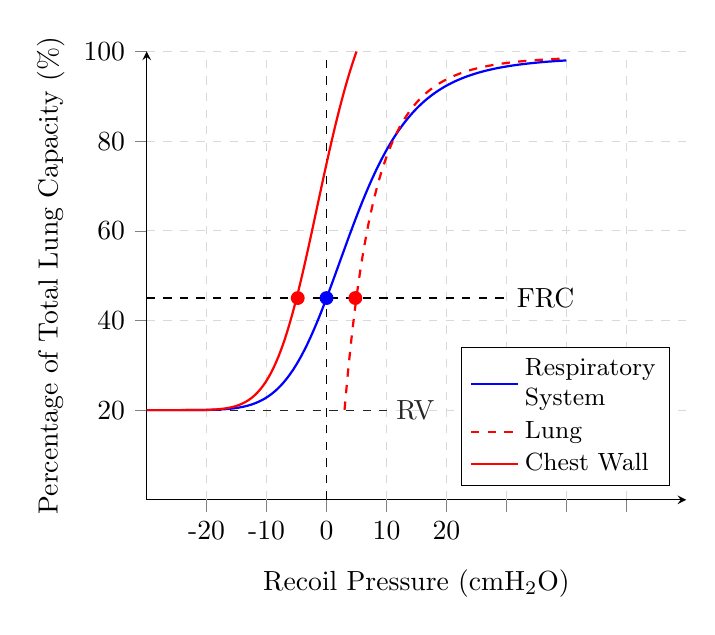
\begin{tikzpicture}


\begin{axis}[
        axis lines=middle,
	ymin = 0,
	ymax = 100,
	xmin = 0,
xmax = 90,
        grid = major,
        grid style={dashed, gray!30},
	 ylabel near ticks,
	xlabel near ticks,
	  xticklabels={},
	extra x ticks={10,20,30,40,50,60,70},
extra x tick labels = {-20,-10,0,10,20},
extra x tick style={draw=none},
        xlabel=Recoil Pressure (cmH\textsubscript{2}O),
        ylabel=Percentage of Total Lung Capacity (\%),
        tick align=outside,
        enlargelimits=false,
legend pos= south east,
legend style={font=\small, cells={align=left}},
legend cell align={left}]

\draw [black, thin, dashed] (axis cs: 30,0) -- (axis cs: 30,100);

\addplot [domain=0:60, thick, black, dashed, forget plot] {45} node[right]{FRC} node[circle,fill=blue,inner sep=0pt,minimum size=5pt, pos=0.5]{} node[circle,fill=red,inner sep=0pt,minimum size=5pt, pos=0.42]{} node[circle,fill=red,inner sep=0pt,minimum size=5pt, pos=0.58]{};
\addplot [domain=0:40, thin, gray!30!black, dashed, forget plot] {20} node[right]{RV};

\plot[domain=0:70, blue, thick,samples=500] {98.86253 + (20 - 98.86253)/(1 + (x/33.93861)^6.222311)};
\addlegendentry{Respiratory \\ System}
\plot[domain=33:70, red, thick, dashed,samples=500] {99.03006 + (-175471700 - 99.03006)/(1 + (x/3.507017)^6.519079)};
\addlegendentry{Lung}
\plot[domain=0:35, red, thick,samples=500] {125.2831 + (20 - 125.2831)/(1 + (x/29.61216)^6.890834))};
\addlegendentry{Chest Wall};


\end{axis}

\end{tikzpicture} 
\end{document}